\section{Experimento 2}

\subsection{Medición de la resistencia serie equivalente de condensadores electrolíticos}

Para el siguiente experimento emplearemos la placa mostrada acontinuación, en la cual podremos montar capacitores y resistencias sin tener que soldarlas, esto para poder cambiar entre tres valores de capacitores electrolíticos distintos y medir la resistencia serie equivalente de cada uno de ellos. 

\begin{figure}[H]
    \centering
    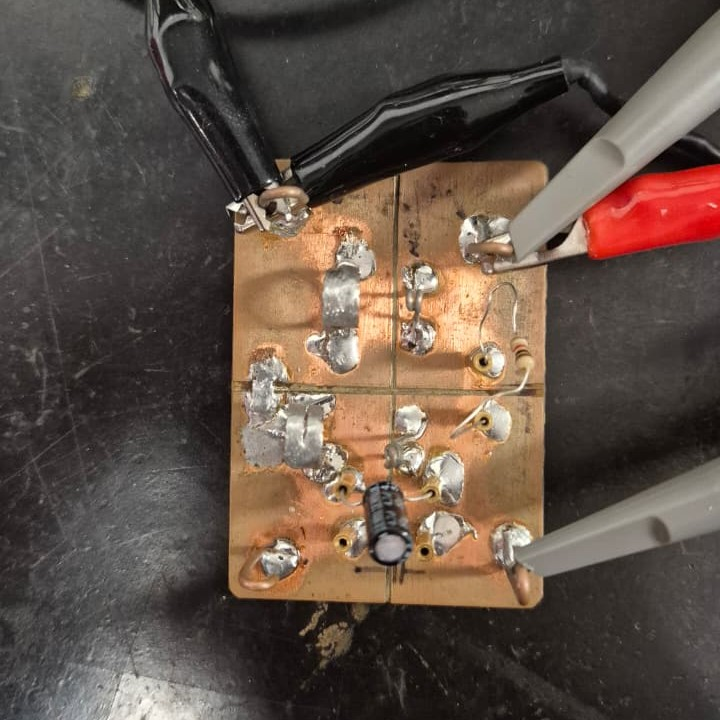
\includegraphics[width=0.4\textwidth]{images/placa2.jpeg}
    \caption{Placa de experimento para la medición de la resistencia serie equivalente de condensadores electrolíticos.}
    \label{fig:placa_experimento2}
\end{figure}

Dicha placa la podemos representar por el siguiente esquema.

\begin{figure}[H]
    \centering
    
\includegraphics[width=0.4\textwidth]{images/esquema2.png}
    \caption{Esquema de la placa de experimento para la medición de la resistencia serie equivalente de condensadores electrolíticos.}
    \label{fig:esquema_placa_experimento2}
\end{figure}

En donde inyectamos una señal cuadrada que nos dara una corriente mostrada en la figura anterior, ademas de los potenciales del capacitor. Buscaremos medir este para poder obtener la resistencia serie equivalente de cada capacitor.\\

Para empeza contectaremos el generador la placa y el osciloscopio de la siguiente manera.


\begin{figure}[H]
    \centering
    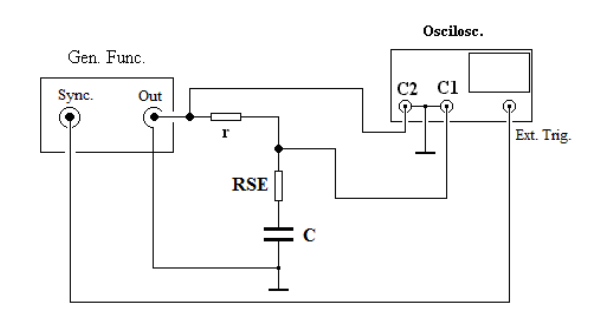
\includegraphics[width=0.4\textwidth]{images/medicion2.png}
    \caption{Esquema de medición}
    \label{fig:conexion_experimento2}
\end{figure}

Como vemos en la figura del esquema de la placa tendremos dos potenciales, el ``eR'' y el ``eC'', pero al estar todo concentrado en el mismo capacitor, nosotros observaremos la suma de ambos potenciales, por lo que buscaremos una figura similar a la de ``eC + eR'' en el osciloscopio. Para poder medir correctamente usamos nuevamente el disparo externo para el osciloscopio y pondremos la punta del Canal 2 en x10, mientras que la del Canal 1 estará en x1 por la baja impedancia del punto de medición.\\

Ahora pasaremos a medir con una resistencia ``r'' de 1 $k\Omega$, y primero un capacitor de 1 $\mu$F, luego uno de 2.2 $\mu$F y por último uno de 4.7 $\mu$F, para esto inyectaremos una señal cuadrada de 10 kHz y en nustro caso usamos 20 Vpp, y ajustaremos la amplitud de la señal para que no se distorsione.\\

Obtendremos la siguiente señal. 



\begin{table}[H]
\resizebox{\columnwidth}{!}{%
\begin{tabular}{|
>{\columncolor[HTML]{FFCE93}}c |c|c|c|}
\hline
f                                                       & 10kHz          & 10kHz          & 10kHz          \\ \hline
C(Nominal)                                              & $1 \mu F$      & $2.2 \mu F$    & $4.7 \mu F$    \\ \hline
r                                                       & $1 k\omega $   & $1 k\omega $   & $1 k\omega $   \\ \hline
\begin{tabular}[c]{@{}c@{}}epp\\ (Canal 2)\end{tabular} & 20Vpp          & 20Vpp          & 20Vpp          \\ \hline
I = epp/r                                               & 20mA           & 20mA           & 20mA           \\ \hline
eR                                                      & 776mV          & 288mV          & 392mV          \\ \hline
RSE = eR/I                                              & $38.8 \omega $ & $14.4 \omega $ & $19.6 \omega $ \\ \hline
\end{tabular}%
}
\end{table}